% !TEX root = report.tex

\subsection{Input file}

Now let's have a look at the input file.

First we see the first input file \texttt{inp1}, with $4$ \ce{Ar} atoms in a FCC cell,
the atom mass is assumed to be \SI{40}{\atomicmassunit},
see Fig. \ref{fig:fcc1} for reference.
\begin{figure}[h]
 \centering
 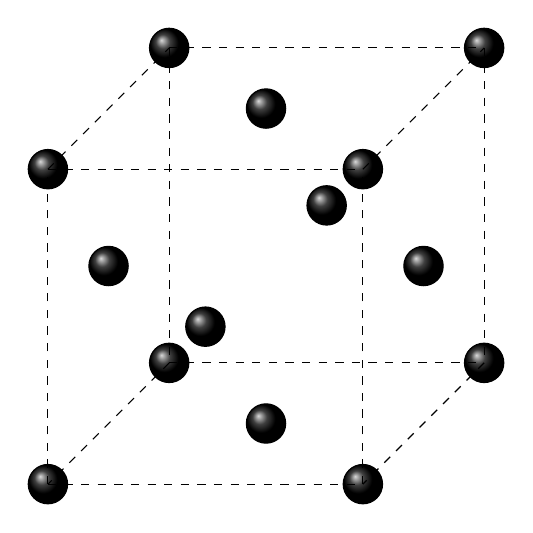
\begin{tikzpicture}
 %points on cube
 \coordinate (A) at (0,0,0);
 \coordinate (B) at (0,0,4);
 \coordinate (D) at (0,4,0);
 \coordinate (C) at (0,4,4);
 \coordinate (E) at (4,0,0);
 \coordinate (F) at (4,0,4);
 \coordinate (H) at (4,4,0);
 \coordinate (G) at (4,4,4);

 %center of faces
 \coordinate (I) at (0,2,2); %center of face ABCD
 \coordinate (J) at (4,2,2); %center of face EFGH
 \coordinate (K) at (2,4,2); %center of face DCGH
 \coordinate (L) at (2,0,2); %center of face ABFE
 \coordinate (M) at (2,2,4); %center of face CBGF
 \coordinate (N) at (2,2,0); %center of face DAEH

 %place non-atom cube corners
 \shadedraw [ball color= black] (A) circle (0.25cm);
 \shadedraw [ball color= black] (C) circle (0.25cm);
 \shadedraw [ball color= black] (F) circle (0.25cm);
 \shadedraw [ball color= black] (H) circle (0.25cm);
 \shadedraw [ball color= black] (B) circle (0.25cm);
 \shadedraw [ball color= black] (D) circle (0.25cm);
 \shadedraw [ball color= black] (E) circle (0.25cm);
 \shadedraw [ball color= black] (G) circle (0.25cm);

 %draw the center of each face
 \shadedraw [ball color= black] (I) circle (0.25cm);
 \shadedraw [ball color= black] (J) circle (0.25cm);
 \shadedraw [ball color= black] (K) circle (0.25cm);
 \shadedraw [ball color= black] (L) circle (0.25cm);
 \shadedraw [ball color= black] (M) circle (0.25cm);
 \shadedraw [ball color= black] (N) circle (0.25cm);

 %draw cube
 \draw [dashed] (A) -- (B);
 \draw [dashed] (B) -- (C);
 \draw [dashed] (C) -- (D);
 \draw [dashed] (D) -- (A);
 \draw [dashed] (E) -- (F);
 \draw [dashed] (F) -- (G);
 \draw [dashed] (G) -- (H);
 \draw [dashed] (H) -- (E);
 \draw [dashed] (A) -- (E);
 \draw [dashed] (B) -- (F);
 \draw [dashed] (C) -- (G);
 \draw [dashed] (D) -- (H);
\end{tikzpicture}

 \caption{A FCC cell of \ce{Ar} for \texttt{inp1}.}
 \label{fig:fcc1}
\end{figure}

Run the simulation code, we derive the following results,
see Fig. \ref{fig:input1} for reference.
\begin{figure}[h]
 \centering
 \begin{minipage}[t]{0.45\textwidth}
  \includegraphics[width=\linewidth]{input1/avec_abc}
  \subcaption{Lattice parameters of \texttt{inp1}. The dashed dot lines are upper and lower
   bound of the lattice parameters. We can see that $a$, $b$, $c$ lines coincide with each
  other.}
  \label{fig:input1:ee}
 \end{minipage}
 \hfil
 \begin{minipage}[t]{0.45\textwidth}
  \includegraphics[width=\linewidth]{input1/t}
  \subcaption{Total energy of \texttt{inp1}. The dashed dot lines are upper and lower
   bound of the total kinetic energy and total potential energy. Total energy is the sum
  of the other two.}
  \label{fig:input1:e}
 \end{minipage}
 \hfil
 \vfill
 \begin{minipage}[t]{0.45\textwidth}
  \includegraphics[width=\linewidth]{input1/a}
  \subcaption{Atomic contribution to total energy of \texttt{inp1}.
   The dashed dot lines are upper and lower bound of the
   total atomic energy. We can see that atoms do not contribute
  to total kinetic energy.}
  \label{fig:input1:a}
 \end{minipage}
 \hfil
 \begin{minipage}[t]{0.45\textwidth}
  \includegraphics[width=\linewidth]{input1/l}
  \subcaption{Lattice contribution to total energy of \texttt{inp1}.
   The dashed dot lines are upper and lower bound of the
   total lattice energy. We can see that lattice do not contribute
  to total potential energy.}
  \label{fig:input1:l}
 \end{minipage}
 \caption{Simulation results for \texttt{inp1}.}
 \label{fig:input1}
\end{figure}
